%!TEX root=../oi-magistr-si.tex
\section[WA2 - Web. architektury, perzistence, WS, messaging]{Vhodnost nasazení jednotlivých webových architektur, sdílení dat, perzistence, webové služby a REST, asynchronnost, messaging.}

\paragraph{Vhodnost nasazení jednotlivých webových architektur}
Toto je podle Klímy spíš diskusní téma, to znamená použít zdravý rozum a být schopen přemýšlet, na co se hodí cloud. Třídy aplikací a způsoby jejich nasazení: desktop, klasické webové aplikace na aplikačním serveru, cloudová řešení.

\priklad Elektronické bankovnictví, které má 20 let starý back-end legacy system naprogramovaný v COBOLu. Klienti přistupují přes webové JEE (JSP) rozhraní. zvážit architekturu systému vzhledem k nárůstu počtu klientů nebo růstu bank, zvážit privátní cloud vs. existující provideři AWS, Google, MS Azure.

Typická architektura (cloudové) aplikace. Je mnoho klientů, kteří interagují například s webovou službou. Ta může být horizontálně škálovatelná (co do počtu serverů). Zde může být i nějaký load balancer, který klienty rovnoměrně přiřazuje méně vytíženým strojům. Služba buď zpracuje požadavek rovnou do databáze (storage), nebo pokud se jedná o nějakou (časově) náročnější akci (například převod fotek atd.), tak tu pošle do fronty ke zpracování. Z fronty si tzv. \uv{worker role} postupně berou jednotlivé úlohy a na pozadí je provádění (opět mohou být horizontálně škálovatelné).

\begin{figure}[h!]
\centering
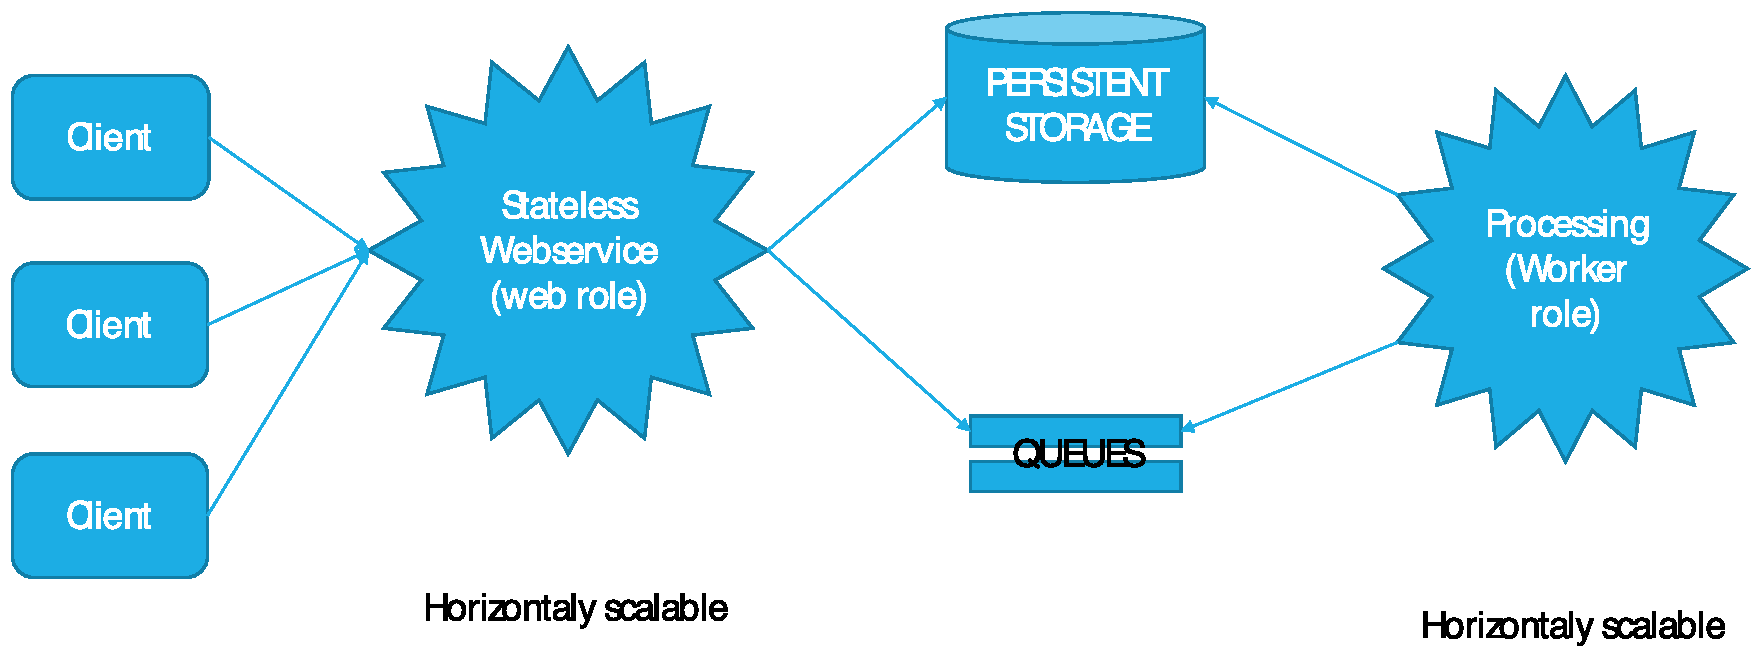
\includegraphics[width=140mm]{17/images/cloud-architecture}
\end{figure}

\subsection{Sdílení dat, persistence}
Hlavně relační DB, protože objektové nejsou moc cool - nevýhody přímého použití JDBC
\paragraph{ORM}
\begin{itemize}[itemsep=0px]
\item Blíže OO paradigmatu
\item JPA - standardizované API pro ORM: implementace např. Hibernate (konfigurace pomocí XML nebo anotacemi)
\item ORM by měl být neintruzivní - pracuje přímo s POJO (implicitní konstruktor, settery a gettery, ne final atributy)
\item podpora ISA (dědění) hierarchie:
    \begin{itemize}[itemsep=0px]
    \item SINGLE\_TABLE - vše v jedné tabulce + rozlišující sloupec
    \item TABLE\_PER\_CLASS - každá entita má vlastní tabulku s celou sadou atributů
    \item JOINED - hlavní tab. má základní attrib., ostatní se s ní spojují (slabé entity)
    \end{itemize}
\item podpora vztahů (1:1, 1:N, M:N)
\item dialekty SQL (snaha o sjednocení SQL syntaxe)
\item perzistenci se starají třídy EntityManager nebo Hibernate Session - operace \texttt{persist, find, merge, remove, query}
\end{itemize}

\subsection{WS a REST}
A web service is a function that can be accessed by other programs over the web (Http). A web service is a collection of open protocols and standards used for exchanging data between applications or systems. Software applications written in various programming languages and running on various platforms can use web services to exchange data over computer networks like the Internet in a manner similar to inter-process communication on a single computer. This interoperability (e.g., between Java and Python, or Windows and Linux applications) is due to the use of open standards (XML, SOAP, HTTP)

\begin{itemize}[itemsep=0px]
\item architektonický styl pro distribuovaná media
\item platformně nezávislé
\item založeno na technologii HTTP a URI
\item cíl: obecné aplikační rozhraní, možnost komunikace přes proxy - manipulace se zdroji (informace, data, soubory)
\item zdroj je identifikován svým URI
\item client-server (aplikační logika rozdělená mezi server a klient),
\item stateless (bezestavová komunikace - jeden požadavek nese všechny informace které server potřebuje k jeho zpracování),
\item pro popis metadat se používají HTTP hlavičky
\item minimalizace závislostí klienta a serveru
\item server může cacheovat odpovědi
\item klient neví, zda komunikuje se serverem nebo prostředníkem (proxy, cache)
\end{itemize}

\subsection{Messaging}
Synchronní (blokující) vs. asynchronní (neblokující) - granularita. Mezi aplikacemi nebo front-endem a back-endem (message driven beans, middleware, webservices, http, REST, sockety, AJAX) slouží zejména ke komunikaci a integraci aplikací. Mezi procesy (fronty) (cloudová řešení jako AWS Simple Queue Service, GAE Task Queue, MS Azure Queue) slouží zejména k dávkovém zpracování velkého množství dat, ale i na posílání jednoduchých zpráv.
